\documentclass[11pt, openright]{book}

    % Cover Variables
	\newcommand{\ctoptitle}{Travaux Pratiques}
	\newcommand{\ctitle}{Interférence et Diffraction}
        \newcommand{\cautor}{Eva Maturana - Lucas Lescure}

    % Header Variables
        \newcommand{\headRE}{\emph{\thepage}}
        \newcommand{\headLE}{\emph{\thesection. \rightmark}}
        \newcommand{\footRE}{}
        \newcommand{\footLE}{}

    % TOC Variables
        \newcommand{\toctitle}{Table des Contenus}
        \newcommand{\tocchapter}{TP}
        \newcommand{\toccount}{3}
  
    % Chapter Variables
        \newcommand{\chvar}{TP}

\usepackage[a4paper, total={16cm, 22.125cm}]{geometry}

% Page Style
\usepackage[]{environ}
% Cover Page 
\usepackage{tikz}
\makeatletter
\def\parsecomma#1,#2\endparsecomma{\def\page@x{#1}\def\page@y{#2}}
\tikzdeclarecoordinatesystem{page}{
    \parsecomma#1\endparsecomma
    \pgfpointanchor{current page}{north east}
    % Save the upper right corner
    \pgf@xc=\pgf@x%
    \pgf@yc=\pgf@y%
    % save the lower left corner
    \pgfpointanchor{current page}{south west}
    \pgf@xb=\pgf@x%
    \pgf@yb=\pgf@y%
    % Transform to the correct placement
    \pgfmathparse{(\pgf@xc-\pgf@xb)/2.*\page@x+(\pgf@xc+\pgf@xb)/2.}
    \expandafter\pgf@x\expandafter=\pgfmathresult pt
    \pgfmathparse{(\pgf@yc-\pgf@yb)/2.*\page@y+(\pgf@yc+\pgf@yb)/2.}
    \expandafter\pgf@y\expandafter=\pgfmathresult pt
}
\makeatother


% Object formatting
\usepackage[12pt]{moresize}
\usepackage[]{anyfontsize}
\usepackage{titlesec}
\usepackage{import}
\usepackage{floatrow}
\usepackage{enumitem}
\usepackage{changepage}
\usepackage[normalem]{ulem}
\usepackage{array}
\newcommand{\ul}[1]{\underline{#1}}

\usepackage[]{chngcntr}
\usepackage{ifthen}
\ifthenelse{\figcountdepth > 1}
  {\counterwithin{figure}{section}\counterwithin{table}{section}}
  {}

\usepackage[format=plain, labelfont=it, textfont=it]{caption}
\makeatletter
\def\@makecaption#1#2{%
    \vskip\abovecaptionskip
    \sbox\@tempboxa{\textit{#1.} #2}

       
   

    \ifdim \wd\@tempboxa >\hsize
        #1. #2\par
    \else
        \global \@minipagefalse
        \hb@xt@\hsize{\hfil\box\@tempboxa\hfil}
    \fi
    \vskip\belowcaptionskip}
\makeatother

\DeclareCaptionFormat{underline}{\uline{#1#2#3}\par}

% Sections
\titleformat{\section}{\fontsize{16}{19.2}\bfseries}{\thesection.}{0.25em}{}
\titleformat{\subsection}{\fontsize{14}{16.8}\bfseries}{\tab\thesubsection.}{0.25em}{}
\titleformat{\subsubsection}{\fontsize{10}{12}}{\uline{\thesubsubsection)\enspace}}{0em}{\uline}





% Geometry

% Typewritting

\setlength{\parskip}{1em}
\setlength{\parindent}{0em}


\newenvironment{items}[3][0pt]
{\def\closesep{#3}
    \vspace{#2}
    \begin{itemize}
        \setlength{\itemsep}{#1}
        \setlength{\topsep}{0pt}
        \setlength{\partopsep}{0pt}}
        {\end{itemize}
    \vspace{\closesep}}

\newenvironment{enum}[3][0pt]
{\defclosesep{#3}
    \vspace{#2}
    \begin{enumerate}
        \setlength{\itemsep}{#1}
        \setlength{\topsep}{0pt}
        \setlength{\partopsep}{0pt}}
        {\end{enumerate}
    \vspace{\closesep}}

\newenvironment{eq}[2]
{\def\closesep{#2}
    \vspace{#1}
    \begin{align*}}
        {\end{align*}
    \vspace{\closesep}}

\newenvironment{lfeq}[2]
{\def\closesep{#2}
    \vspace{#1}
    \begin{flalign*}}
        {\end{flalign*}
    \vspace{\closesep}}
% List Formatting


\NewEnviron{dent}[1]{
    \vspace{-10pt}
    \begin{adjustwidth}{7mm}{}
        \uline{#1}\hspace{2mm}
        \BODY
    \end{adjustwidth}
    \vspace{-10pt}
}


\usepackage[framemethod=tikz]{mdframed}
\newcounter{count_theorem}[section]\setcounter{count_theorem}{0}
\newcommand{\thetheorem}{\arabic{count_theorem}}

\newcounter{count_exercise}[section]\setcounter{count_exercise}{0}
\newcommand{\theexercise}{\arabic{count_exercise}}


\newenvironment{theorem}[1][]{
    \refstepcounter{count_theorem}
    \mdfsetup{
        linecolor=red!30,
        innerbottommargin=10pt,
        linewidth=2pt,
        topline=false,
        bottomline=false,
        rightline=false,
        shadow=true,
        shadowsize=4.5pt,
        frametitlerule=false,
        apptotikzsetting={
                \tikzset{
                    mdfbackground/.append style={
                            left color=red!8,right color=red!3
                        }
                }
            }
    }
    \begin{mdframed}[]\relax
        \ifstrempty{#1}
        {\textbf{Theorem~\thetheorem.} }
        {\textbf{Theorem~\thetheorem.~#1} }
        }
        {\end{mdframed}\vspace{-10pt}
}

\newenvironment{note}{
    \mdfsetup{innertopmargin=5pt,
        linecolor=gray!30,
        linewidth=2pt,
        topline=false,
        bottomline=false,
        rightline=false,
        frametitleaboveskip=0pt,
        shadow=false,
        shadowsize=4pt,
        frametitlerule=false,
        apptotikzsetting={
                \tikzset{
                    mdfbackground/.append style={
                            left color=gray!8,right color=gray!3
                        }
                }
            }
    }
    \begin{mdframed}[]\relax
        \textbf{Note. }
        }
        {\end{mdframed}\vspace{-10pt}
}

\newenvironment{example}{
    \mdfsetup{innertopmargin=5pt,
        linecolor=green!30,
        linewidth=2pt,
        topline=false,
        bottomline=false,
        rightline=false,
        frametitleaboveskip=0pt,
        shadow=false,
        shadowsize=4pt,
        frametitlerule=false,
        apptotikzsetting={
                \tikzset{
                    mdfbackground/.append style={
                            left color=green!7,right color=green!2
                        },
                    mdfframetitlebackground/.append style={
                            left color=green!7,right color=green!2
                        }
                }
            }
    }
    \begin{mdframed}[]\relax
        \textbf{Example. }
        }
        {\end{mdframed}\vspace{-10pt}
}


\usetikzlibrary{calc,arrows}

\tikzset{
    excursus arrow/.style={%
            line width=2pt,
            draw=gray!40,
            rounded corners=2ex,
        },
    excursus head/.style={
            fill=white,
            font=\bfseries\sffamily,
            text=gray!80,
            anchor=base west,
        },
    excursus line/.style={%
            line width=2pt,
            draw=gray!40,
            rounded corners=2ex,
        }
}

\newenvironment{exercise}[1][]{%
    \refstepcounter{count_exercise}
    \mdfsetup{
        singleextra={
                \path let \p1=(P), \p2=(O) in (\x2,\y1) coordinate (Q);
                \path let \p1=(Q), \p2=(O) in (\x1,{(\y1-\y2)/2}) coordinate (M);
                \path [excursus line] ($(O)+(5em,0ex)$) -| (M) |- ($(Q)+(20em,0ex)$);
                \node [excursus head] at ($(Q)+(2.5em,-0.75pt)$) {\ifstrempty{#1}{Exercise \theexercise}{Exercise \theexercise:~#1}};},
        firstextra={
                \path let \p1=(P), \p2=(O) in (\x2,\y1) coordinate (Q);
                \path [excursus arrow,-to] (O) |- ($(Q)+(12em,0ex)$) .. controls +(0:16em) and +(185:6em) .. ++(23em,2ex);},
        middlelinewidth=2.5em,middlelinecolor=white,
        hidealllines=true,topline=true,
        innertopmargin=0.5ex,
        innerbottommargin=2.5ex,
        innerrightmargin=2pt,
        innerleftmargin=2ex,
        skipabove=0.87\baselineskip,
        skipbelow=0.62\baselineskip,
    }
    \begin{mdframed}[]\relax}
        {\end{mdframed}\vspace{-10pt}
}

% Functions and Data Plotting
\usepackage{subfig,wrapfig,adjustbox,multirow}


% Plotting Style
\usepackage{graphicx,pgfplots}
\usetikzlibrary{arrows}
\usetikzlibrary {patterns,patterns.meta}
\usepgfplotslibrary{fillbetween}
\pgfplotsset{compat=1.18}

\usepgfplotslibrary{units}
% Logarithmic Scale
\pgfplotsset{
    log x ticks with fixed point/.style={
            xticklabel={
                    \pgfkeys{/pgf/fpu=true}
                    \pgfmathparse{exp(\tick)}%
                    \pgfmathprintnumber[fixed relative, precision=3]{\pgfmathresult}
                    \pgfkeys{/pgf/fpu=false}
                }
        }
}


% Mathematics

% Formatting
\usepackage{amsmath}
\usepackage{esvect}
\usepackage{amsfonts}
\usepackage{tasks,environ}
\usepackage{xargs}
\usepackage{esint}
\usepackage[]{listings}


\usepackage[english]{babel}
\usepackage{amsthm}
%\newtheorem{theorem}{Theorem}
%\newtheorem{proof}{Proof}



%Custom Shortcuts
\newcommand{\eqi}{\Leftrightarrow}
\newcommand{\lr}[1]{\left( #1 \right)}
\newcommand{\limit}[1]{\displaystyle{\lim_{#1}}}
\newcommand{\tab}{\hspace*{7mm}}
\newcommand{\ds}[1]{\displaystyle{#1}}
\newcommand{\floor}[1]{\lfloor #1 \rfloor}
\newcommand{\R}{\mathbb{R}}
\newcommand{\N}{\mathbb{N}}
\newcommand{\Z}{\mathbb{Z}}
\newcommand{\C}{\mathbb{C}}
\newcommand{\K}{\mathbb{K}}
\newcommand{\F}{\mathcal{F}}
\newcommand{\M}{\mathcal{M}}
\renewcommand{\l}{\lambda}
\newcommand{\seg}[1]{\overline{\rm {#1}}}
\newcommand{\Int}{\int\limits}
\newcommand{\ex}{\tab \uline{Example :}\hspace{0.2cm} }
\newcommand{\vard}{\partial}
\newcommand{\Q}{\mathcal{Q}}
\newcommand{\Vect}{\operatorname{Vect}}
\newcommand{\rg}{\operatorname{rg}}
\renewcommand{\dim}{\operatorname{dim}}
\renewcommand{\Re}{\operatorname{Re}}
\renewcommand{\Im}{\operatorname{Im}}
\renewcommand{\P}{\mathcal{P}}
\newcommand{\blr}[1]{\left\{#1\right\}}
\newcommand{\linecenter}[1]{\par\vspace{2mm} \centerline{#1}\par\vspace{-2mm}}
\newcommand{\dd}{\textrm{d}}
\newcommand{\supp}{\operatorname{Supp}}
\renewcommand{\vec}{\overrightarrow}
\renewcommand{\epsilon}{\varepsilon}

% Matrix Configurations

\makeatletter
\renewcommand*\env@matrix[1][*\c@MaxMatrixCols c]{%
    \hskip -\arraycolsep
    \let\@ifnextchar\new@ifnextchar
    \array{#1}}
\makeatother


% Colors
\usepackage{xcolor}
\newcommand{\blu}{\color{blue}}
\newcommand{\Red}{\color{red}}
\newcommand{\blac}{\color{black}}

\newcommand{\red}[1]{\textcolor{red}{#1}}

\usepackage{xcolor,xspace}
\usepackage{breqn}


% Headings  
\usepackage[Glenn]{fncychap}
\ChNumVar{\fontsize{40}{42}}
\ChTitleVar{\Large\sc}
\ChNameVar{\Large\sc}
\setlength\headheight{14.5pt}
\renewcommand\FmN[1]{\chvar}



\usepackage{fancyhdr}
\usepackage{ragged2e}

% Header & Footers
\renewcommand{\chaptermark}[1]{\markboth{#1}{#1}}
\renewcommand{\sectionmark}[1]{
    \markright{ #1}
}
\pagestyle{fancy}
\fancyhf{}
\fancyhead[LE,RO]{\headLE}
\fancyhead[RE,LO]{\headRE}
\fancyfoot[LE,RO]{\footLE}
\fancyfoot[RE,LO]{\footRE}
\renewcommand{\headrulewidth}{0.5pt}
\fancyheadoffset{1cm}

\fancypagestyle{plain}{%
    \fancyhf{} % clear all header and footer fields
    \fancyfoot[LE, RO]{\footLE}
    \renewcommand{\headrulewidth}{0pt}
    \renewcommand{\footrulewidth}{0pt}}


\fancypagestyle{nohead}{%
    \fancyhf{} % clear all header 
    \fancyfoot[LE, RO]{\footLE}
    \fancyfoot[LO, RE]{\footRE}}

    \fancypagestyle{head}{%
    \fancyhf{} % clear all header 
    \fancyhead[LE,RO]{\headLE}
\fancyhead[RE,LO]{\headRE}
\renewcommand{\headrulewidth}{0.5pt}
\fancyheadoffset{1cm}
    }


\fancypagestyle{bib}{%
    \fancyhf{} % clear all header and footer fields
    \fancyhead[CE, CO]{}
    \fancyfoot[LE, RO]{\footLE}
    \fancyfoot[LO, RE]{Bibliographie}}

% Table of Contents

\renewcommand*\thechapter{\arabic{chapter}} %Usually Roman
\renewcommand*\thesection{\arabic{section}}
\renewcommand*\thesubsubsection{\thesubsection.\alph{subsubsection}}
\makeatletter
\@removefromreset{section}{chapter}
\makeatother


% Table of Contents

\usepackage{titletoc}
\usepackage{ erewhon,cabin}
\usepackage[linktoc=all]{hyperref}
\renewcommand*\contentsname{\centerline{\toctitle}}

\setcounter{secnumdepth}{3}
\setcounter{tocdepth}{\toccount}

\usepackage[subfigure]{tocloft}
\setlength\cftparskip{0pt}

\usepackage{etoolbox}
\makeatletter
\pretocmd{\chapter}{\addtocontents{toc}{\protect\addvspace{5\p@}}}{}{}
\pretocmd{\section}{\addtocontents{toc}{\protect\addvspace{-10\p@}}}{}{}
\pretocmd{\subsection}{\addtocontents{toc}{\protect\addvspace{1\p@}}}{}{}
\makeatother


% Chapter Style
\titlecontents{chapter}
[11em]
{\bigskip}
{\bfseries\textsc\tocchapter~\textsc\thecontentslabel : \textsc}
{\hspace*{-5.5em}\textbf}
{\titlerule*[1pc]{ }}[\smallskip]

% Section Style
\titlecontents{section}
[0em] % i
{\bigskip\bfseries}
{\fontsize{11}{13.2}\bfseries\uline{\thecontentslabel.\enspace}\uline}
{\hspace*{-4em}\textbf}
{\hspace{0.5pt}\uline{\hspace*{\fill}}\contentspage}

% Subsection Style
\titlecontents{subsection}
[2em] % i
{\smallskip\bfseries}
{\fontsize{10}{12}\bfseries\thecontentslabel.\enspace}
{\hspace*{-4em}}
{\titlerule*[0.5pc]{.}\contentspage}

% Subsubsection Style
\titlecontents{subsubsection}
[4em] % i
{\smallskip}
{\fontsize{10}{12}\thecontentslabel)\enspace}
{\hspace*{-4em}}
{\titlerule*[0.5pc]{.}\contentspage}










    % figure support
	\usepackage{import}
	\usepackage{xifthen}
	\pdfminorversion=7
	\usepackage{pdfpages}
	\usepackage{transparent}
	\newcommand{\incfig}[1]{%
            \def\svgwidth{\columnwidth}
            \import{./figures/}{#1.pdf_tex}
	}

	\pdfsuppresswarningpagegroup=1

	\makeatletter
\@addtoreset{section}{chapter}
\makeatother  

\begin{document}
    % Spacing
        % Section Spacing
\titlespacing\section{0pt}{3pt plus 2pt minus 2pt}{6pt plus 2pt minus 1pt}
\titlespacing\subsection{0pt}{0pt plus 1pt minus 1pt}{0pt plus 3pt minus 1pt}
\titlespacing\subsubsection{0pt}{0pt plus 0pt minus 0pt}{0pt plus 2pt minus 0pt}

\usetikzlibrary{shadows}

\newgeometry{left=2.5cm, width=16cm, bottom=2.5cm, top=2.5cm}






    % Cover
        % Cover
\definecolor{ccolor1}{RGB}{236,145,143}
\definecolor{ccolor2}{RGB}{131,168,192}
\definecolor{ccolor3}{RGB}{182,227,150}
\definecolor{ccolor4}{RGB}{171,206,145}

\usetikzlibrary{fadings}

\begin{titlepage}
    \newgeometry{top=1cm, width=21cm, bottom=1cm}

    \begin{tikzpicture}[remember picture,overlay,every node/.style={anchor=center}]

        \coordinate (Center) at (page cs: 0,-0.5);
        %F4E Logo
        \begin{scope}[scale = 1.5]
            \foreach \angle in {0,30,...,330} {
                    \filldraw[orange!50!yellow,line width=0.01pt,shift=(Center)] (\angle:3.8637) -- (\angle+30:3.8637) -- (0,0) -- (\angle:3.8637);
                    \draw[white, line width = 7pt,shift=(Center)] (\angle:2cm) arc (\angle-60:\angle:2cm);
                    \draw[white, line width = 7pt,shift=(Center)] (\angle+30:2cm) arc (\angle+90:\angle+30:2cm);
                }
            % Outer delimiter
            \foreach \angle in {15,45,...,345} {
                    \filldraw[white, line width = 7pt,shift=(Center)] (\angle:3.8637cm) arc (\angle-15:\angle+45:2cm) arc (\angle+15:\angle-15:2cm) arc (\angle+45:\angle+15:2cm);
                }
            % Inner delimiter
            \foreach \angle in {15,45,...,345} {
                    \filldraw[white, line width = 7pt,shift=(Center)] (\angle:1.0353cm) arc (\angle-75:\angle-45:2cm) arc (\angle+75:\angle+105:2cm) -- (0,0) -- (\angle:1.0353cm);
                }
            % Stars
            \foreach \angle in {0,30,...,330} {
                    \fill[orange!50!yellow,shift=(Center)] (\angle:1.03527cm) -- ++ (231:0.175) -- ++ (33:0.35) -- ++ (177:0.35) -- ++ (321:0.35) -- ++ (105:0.35) -- ++ (249:0.35) -- ++ (33:0.35);
                }
        \end{scope}

        \node[opacity =0.07, inner sep=0pt, anchor=east] at (current page.east){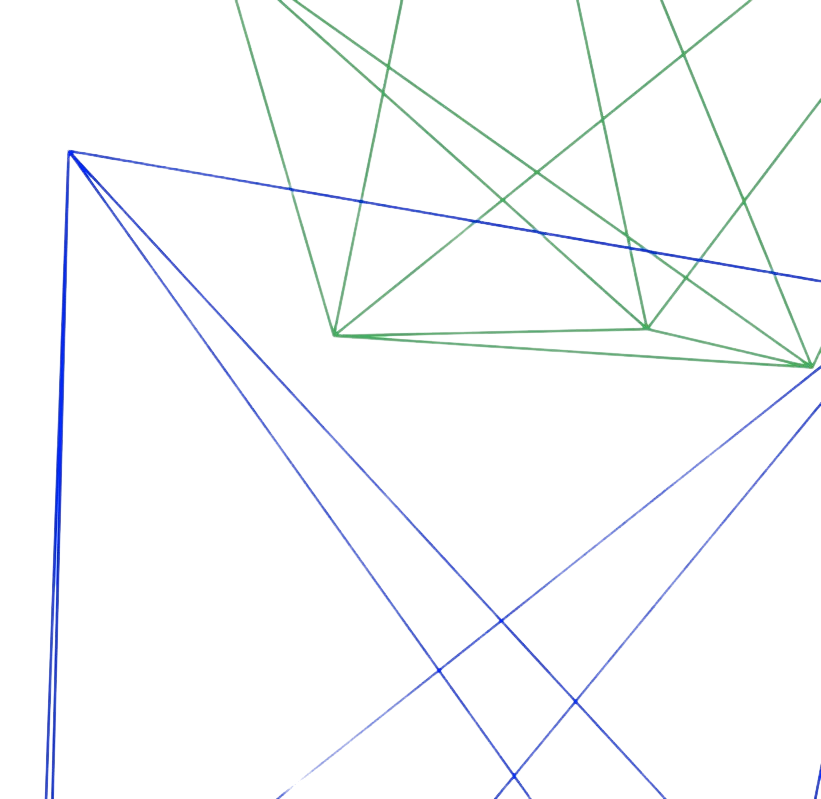
\includegraphics[width=0.5\paperwidth,height=\paperheight]{/root/.config/latex-utils/logos/invert1.png}};

        \node[opacity=0.07,inner sep=0pt, anchor=north west] at (current page.north west){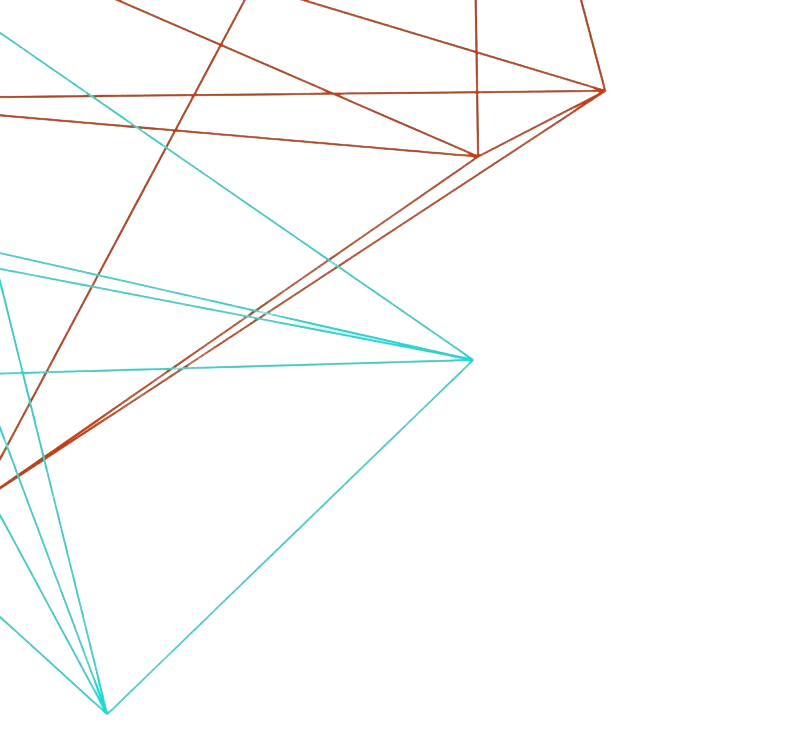
\includegraphics[width=0.5\paperwidth,height=0.5\paperheight]{/root/.config/latex-utils/logos/invert3.png}};




        \node at (page cs:0,0.345) {\Large\textsc{High School Observation and Learning Internship}};
        \node at (page cs:0,0.875) {\Large\bfseries\textsc{Observation Internship}};
        \node at (page cs:0,0.925) {\LARGE\bfseries\textsc{Lycée Français de Barcelone}};

        \node at (page cs:0.5,0) {\Large\textsc{Cyril Lescure - Pedagogical Tutor}};








        %\node[opacity=0.15, inner sep=0pt, anchor=south west] at (current page.south west){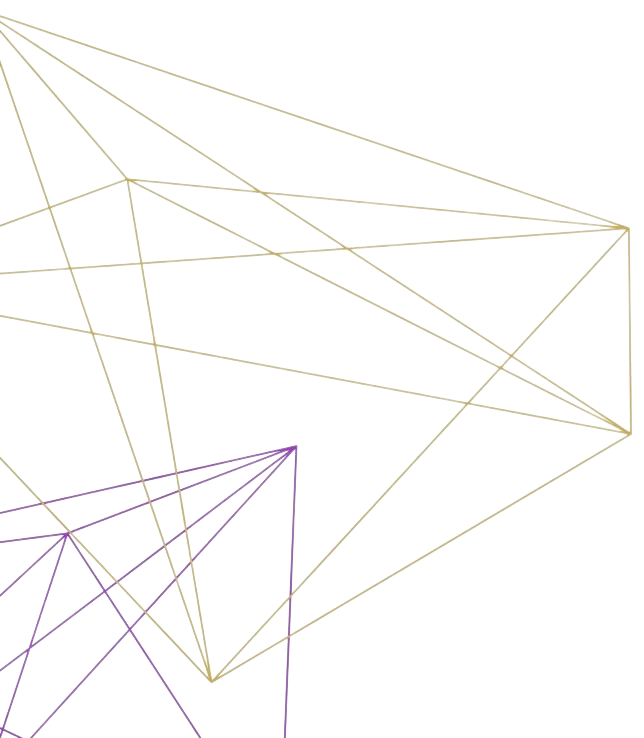
\includegraphics[width=0.5\paperwidth,height=0.5\paperheight]{/root/.config/latex-utils/logos/invert2.png}};

        \node at (page cs:0,0.5) {\fontsize{28}{28.8}\textbf{\ctoptitle}};
        \node at (page cs:0,0.425) {\fontsize{28}{28.8}\textbf{\ctitle}};
        \draw (page cs:0.5,0.375) -- (page cs:-0.5,0.375);
        \node at (page cs:0,0.245) {\LARGE\textsc{\cautor}};
        \node at (page cs:0,0.310) {\Large\textsc{03.06.2019 - 07.06.2019}};


    \end{tikzpicture}
\end{titlepage}


\newgeometry{width=18.625cm, bottom=2cm, top=2cm}

\tikz[remember picture, overlay] \node[opacity=0.3,inner sep=0pt, anchor=north east] at (current page.north east){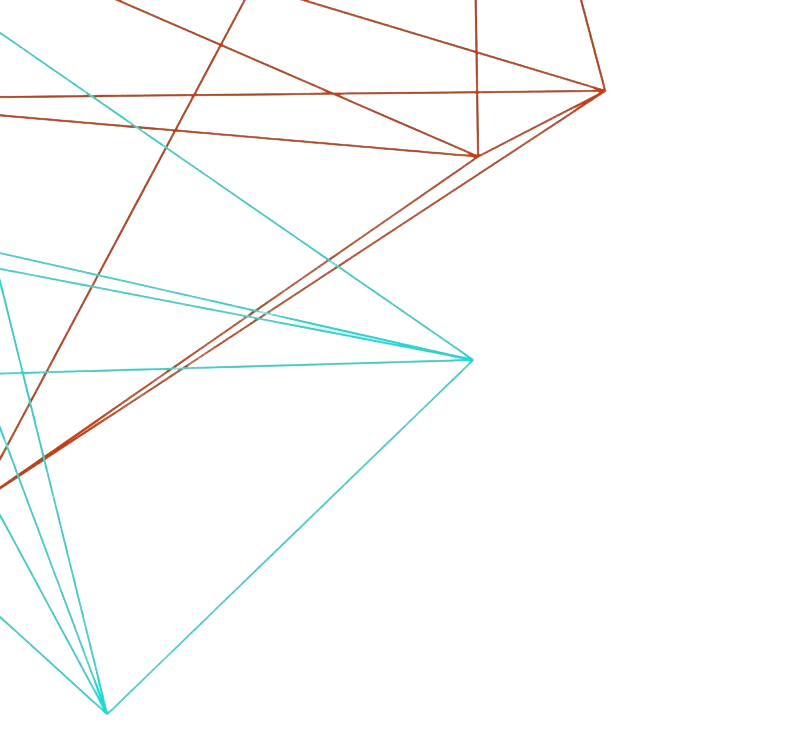
\includegraphics[angle=-90,origin=c,width=0.5\paperheight,height=0.5\paperwidth]{/root/.config/latex-utils/logos/invert3.png}};
\tikz[remember picture,overlay] \node[opacity=0.3,inner sep=0pt, anchor=south east] at (current page.south east){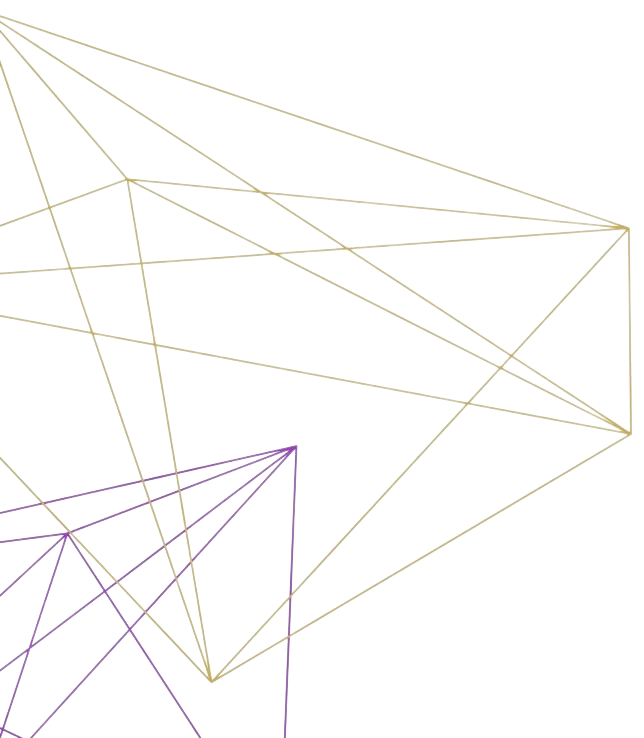
\includegraphics[angle=90,width=0.5\paperwidth,height=0.5\paperheight]{/root/.config/latex-utils/logos/invert2.png}};

\tableofcontents





	
    \newpage
	
	\chapter{Interférences de deux sources}

	\vspace{-2cm}
	\textit{Tout au long du TP on s'assurera d'utiliser une pige de bois de longueur $20\pm 0.1\ cm$ pour determiner les erreurs de mesure entre la position des composant sur l'axe optique et la position des support sur le banc optique}
		

		\section{Introduction}
			
			Quand on superpose deux ondes lumineuses monochromatiques cohérentes de même couleur, elles interfèrent, c'est à dire que la distribution d'intensité résultante de leur superposition dans l'espace n'est pas simplement la somme des distributions d'intensités des deux ondes. On observe en effet dans ce cas une distribution d'intensité  avec des minima dus au phénomènes d'interférences des ondes lumineuses [Figure 1.1].\\
			Pour obtenir deux sources temporellement cohérentes on peut utiliser deux points d'un front d'onde qui provient d'une source unique $S$. Pour le principe d'Huygens en effet ces deux points seront des sources secondaires, $S_1$ et $S_2$, d'ondes sphériques temporellement cohérentes entres elles.\\
			Expérimentalement, les deux sources peuvent être réalisées par exemple en filtrant spatialement deux petites zones différentes d'un front d'onde plan, à l'aide de deux trous ou de deux fentes. Le schéma d'un tel dispositif experimental est montré dans la Figure 1.1.

			\begin{figure}[ht!]
				\centering
				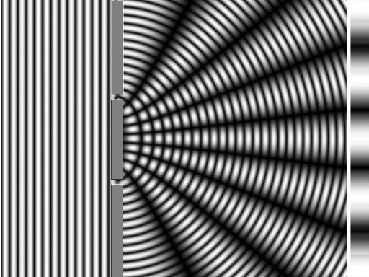
\includegraphics[width=0.4\textwidth]{./object/g1.png}
				\caption{Interférence dans l'espace de deux sources cohérentes générées à l'aide des fentes de Young}
			\end{figure}

		\section{Fentes de Young}

			\subsection{Rappel théorique}
				
				Sur un écran positionné à une distance $D\gg d$, avec $d$ la distance antre les deux fentes en condition de Fraunhofer, on observera une figure d'interférence donné par : \\
				\centerline{$\ds{I(y)=I_0\cos^2\left( \frac{y}{i}\pi \right) }$}
				Où $I_0$ est l'intensité des franges brillantes et $i$, donnés par $\ds{i=\frac{\lambda D}{d}}$

				\begin{figure}[ht!]
					\centering
					\begin{tikzpicture}
						\draw[thick, dashed, gray, -Latex] (-7,0) -- (7,0);
						\draw[thick, -Latex] (-5,-2) -- (-5,2);
						\draw[thick, -Latex] (5,-2) -- (5,2);
						\filldraw[fill = gray] (-4.9,-1.7) -- (-4.9,-0.6) -- (-5.1,-0.6) -- (-5.1,-1.7);
						\filldraw[fill = gray] (-4.9,1.7) -- (-4.9,0.6) -- (-5.1,0.6) -- (-5.1,1.7);
						\filldraw[fill = gray] (-4.9,0.5) -- (-4.9,-0.5) -- (-5.1, -0.5) -- (-5.1,0.5) -- (-4.9,0.5);

						\draw[thin] (-5,0.55) -- (5,1.25);
						\draw[thin] (-5, -0.55) -- (5,1.25);
						\draw[gray, thin] (-5,0) -- (5,1.25);
						
						\draw[Latex-Latex, semithick, gray] (-4.9,-1.3) -- (5,-1.3);
						\draw[Latex-Latex, semithick, gray] (-5.3, 0.6) -- (-5.3, -0.6);

						\draw[semithick] (-3,0) arc (0:7.125:2);

						\node at (-5.3,2) {$x$};
						\node at (4.7,2) {$y$};
						\node at (-2.7,0.15) {$\alpha $};
						\node at (0,-1.6) {$D\gg d$};
						\node at (7,-0.3) {$z$};
						\node at (-5.6,0.3) {$d$};

						\node at (5.75,-1.9) {Écran};
						\node at (-3.25,1.9) {Fentes de Young};



					\end{tikzpicture}
					\caption{Montage pour la réalisation de l'expérience de Young à l'aide d'une source laser}
				\end{figure}


				\subsection{Mesures}

				Pour cette manipulation  on utilisera une source laser monochromatique ($\lambda =632.8\ nm$); cela permet la mise en place du montage expérimental simple, montré dans la Figure 2.1, pour la réalisation de l'expérience de Young.

				On positionne la diapositive avec les fente de Young sur le chemin du laser et on place un écran à $D=51.7\pm 0.1\ cm$. 

				On repère alors une figure d'interférence sur laquelle on mesure l'interfrange $\ds{i_{int} = 1.12 \pm 0.03\  mm}$.\footnote{Trouvé en remplaçant l'ecran par une barrete CCD (données en annexe)} 


				On en déduis alors par la relation $\ds{d=\frac{\lambda  D}{i_{int}}}$ que la séparation des deux fente est $d=28.9\pm 13.4\ \mu m$.\footnote{On veille à utiliser la propagation des incertitudes mise en annexe}

				De plus si l'on masque une des fentes de Young on constate alors la disparition des franges, on a alors une distribution lisse provoqué par la diffraction de la seule fente restante comme ci-dessous sur la Figure 2.2.

				\begin{figure}[ht!]
					\centering
					\begin{tikzpicture}
						\node[overlay, opacity=0.6] at (0,1.95) {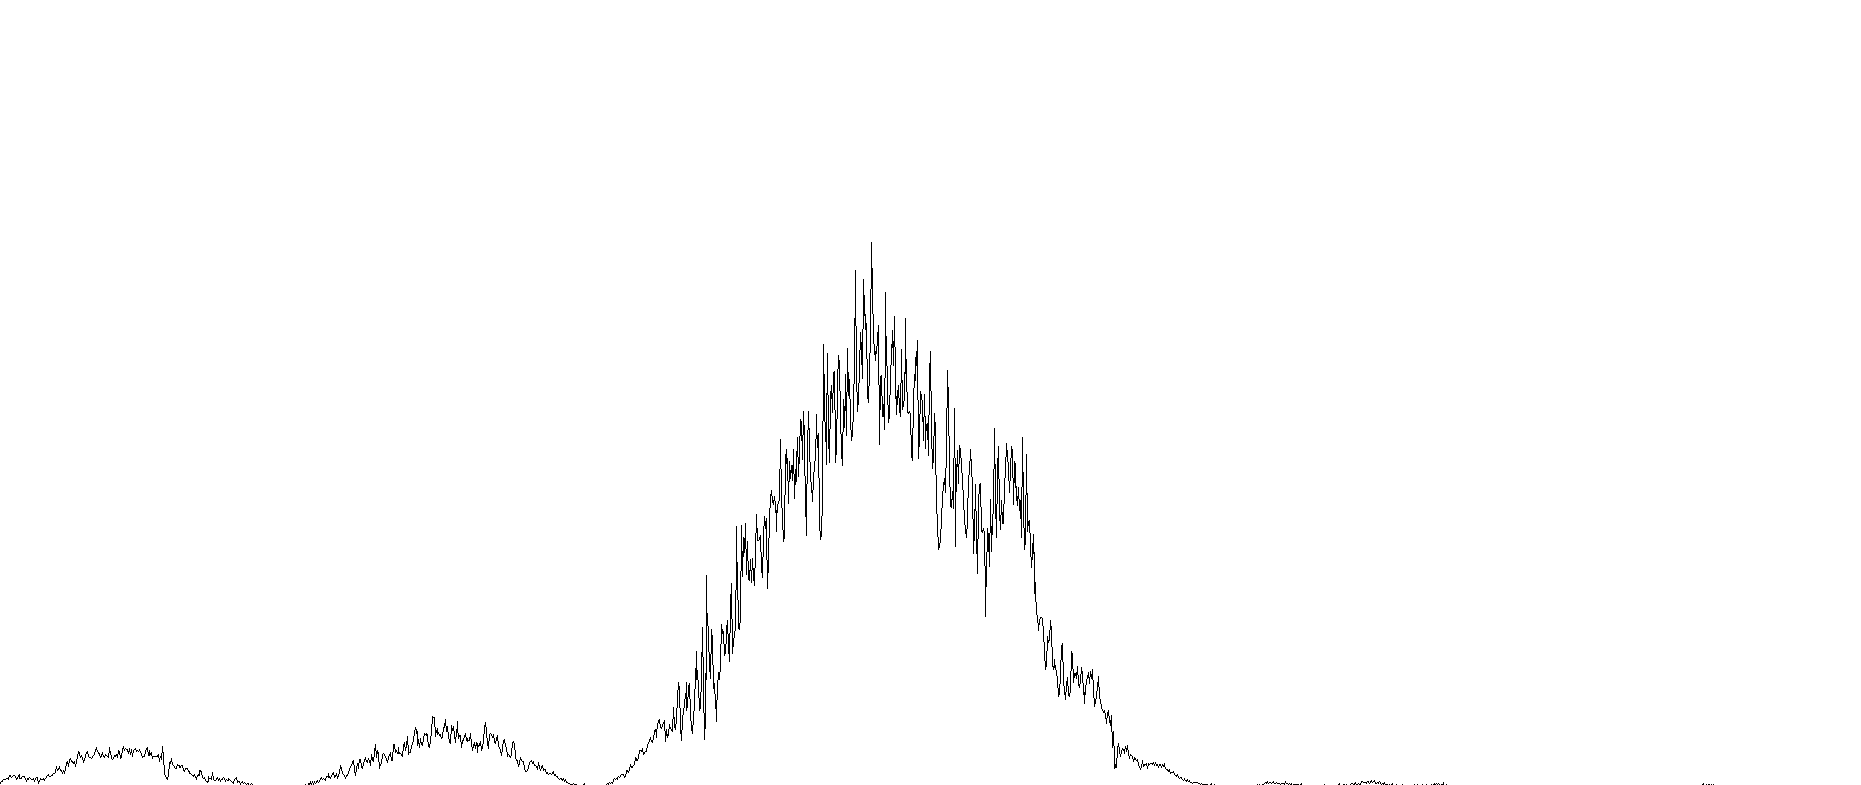
\includegraphics[width=0.495\textwidth]{./object/g2.png}};

						\filldraw[smooth,samples=200,domain=-5:1.6, variable=\x,fill opacity=0.2, fill=red, red] plot({\x},{4.5*((sin(109.5*\x)/(1.91*\x))^2});

						\draw[thick, -Latex] (-5,0) -- (5,0);
						\draw[thick, -Latex] (0,0) -- (0,5);

						\draw (1.64,0.1) -- (1.64,-0.1);
						\draw (0,0) -- (0,-0.1);

						\draw[Latex-Latex,semithick] (-1.64,-0.2) -- (0,-0.2);

						\node at (0.4,5) {$I$};
						\node at (5,0.4) {$y$};

						\node at (-0.83,-0.5) {$4.69 \pm 0.47\ mm$};

					\end{tikzpicture}
					\caption{Distribution d'intensité sur l'écran observé en masquant l'une des fentes}
				\end{figure}

				Cette figure ne peut pas être complètement décrite par les equations vu en \textbf{2.1}. Une description complète doit tenir compte du fait que chaque fente a une largeur $a\neq 0$ et donc elle provoque de la diffraction. Elle se modélise par: \\
				\centerline{$\ds{I(y)=I_0\operatorname{sinc}^2\left( \frac{y}{i_{diff}} \right) }$}
				Où $i_{diff}$ est l'interfrange observée en masquant l'une des fentes s'exprimant : $\ds{i_{diff}=\frac{\lambda  D}{a}}$

				En mesurant la taille de l'interfrange dans la distribution de diffraction on peut determiner la largeur des fentes comme étant $\ds{a=\frac{\lambda D}{i_{diff}}}$, soit $\ds{a=6.98\pm \ 0.84\mu m}$

				On remarque que l'incertitude relative de la mesure est de $12\ \%$, pour remedier ceci on peut augmenter le contraste avec un laser d'intensité plus puissante, pour pouvoir mieux voir les interfranges. Mais on peut aussi essayer d'éloigner l'écran des fentes de Young de façon à avoir une meilleure mesure de l'interfrange.\\
				Il faut cependant veiller à ne pas être trop loins car l'intensité baisse celon ${r^{-2}}$ et donc se perdre dans le bruit de fond.

		\section{Interférence de deux sources ponctuelles par biprisme de Fresnel}
				
			\subsection{Le biprisme de Fresnel}

			Pour générer deux sources ponctuelles cohérentes, $S_1$ et $S_2$, à partir d'une source unique $S$, on peut utiliser un composant optique appelé le 'biprisme de Fresnel'. Il s'agit d'une pièce de verre polie, ayant une section équivalente à deux prismes, d'angle au sommet $\alpha $, accolés par leurs bases [Figure 3.1]. Les sources $S_1$ et $S_2$ sont les images virtuelles de $S$ à travers chacun des prismes.

			\begin{figure}[ht!]
				\centering
				\begin{tikzpicture}
					\draw[thick,dashed, -Latex] (-7,0) -- (7,0);
					\draw[dashed,gray] (-6.5,-2.5) -- (-6.5,2.5);
					\draw[dashed,gray] (-3,-2.5) -- (-3,2.5);
					\draw[very thick] (6,-2.5) -- (6,2.5);

					\filldraw[fill=cyan,very thick, opacity=0.3] (-3,1.75) -- (-2.7,0) -- (-3,-1.75) -- (-3,1.75);

					\filldraw[fill=green, fill opacity=0.15, thin] (-6.5,0) -- (-2.85,1) -- (6,1.5) -- (6,-0.5) -- (-2.75,0.4) -- (-6.5,0);
					\filldraw[fill=cyan, fill opacity =0.15, thin] (-6.5,0) -- (-2.85,-1) -- (6,-1.5) -- (6,0.5) -- (-2.75,-0.4) -- (-6.5,0);
					
					\draw[dashed,thin,gray] (-6.5,0.8) -- (-2.85,1);
					\draw[dashed,thin,gray] (-6.5,0.8) -- (-2.75,0.4);
					\draw[dashed,thin,gray] (-6.5,-0.8) -- (-2.85,-1);
					\draw[dashed,thin,gray] (-6.5,-0.8) -- (-2.75,-0.4);

					\draw[dashed,thin,gray] (-2.85,1) -- (-1,1.5);
					\draw[dashed,thin,gray] (-2.75,0.4) -- (-1,0.6);
					\draw[dashed,thin,gray] (-2.85,-1) -- (-1,-1.5);
					\draw[dashed,thin,gray] (-2.75,-0.4) -- (-1,-0.6);

					\draw[Latex-Latex,semithick] (-6.5,-1.5) -- (-3,-1.5);
					\draw[Latex-Latex,semithick] (-6.5,-2) -- (6,-2);

					\filldraw[fill=black] (-6.5,0) circle (1.75pt);
					\filldraw[color=gray] (-6.5,0.8) circle (1.75pt);
					\filldraw[color=gray] (-6.5,-0.8) circle (1.75pt);

					\draw[thin] (-1.55, 1.35) arc (15:6:1.85);
					\draw[thin] (-1.55, -1.35) arc (-15:-6:1.85);

					\node at (-6.9,0.2) {$S$};
					\node at (-6.8,1) {$S_1$};
					\node at (-6.8,-1) {$S_2$};

					\node at (-4.85,-1.25) {$\Delta $};
					\node at (0,-2.3) {$D\gg d$};

					\node at (-1.11,1.27) {$\theta$};
					\node at (-1.11,-1.27) {$\theta$};

					\node at (5.25,2.5) {Écran};

					\node at (-6.3,0.4) {$\frac{d}{2}$};
					\node at (-6.3,-0.4) {$\frac{d}{2}$};

					\filldraw[fill=cyan, opacity=0.2] (7.5, 2.625) -- (7.95,0) -- (7.5,-2.625) -- (7.5, 2.625);

					\draw[] (7.5,0.75) arc (-90:-80:1.875); 
					\node at (7.7,0.5) {$\alpha $};
					
					\draw[semithick,gray, Latex-Latex] (7.3, 0) -- (7.3, 2.625);
					\node at (7.1,1.3) {$h$};
					\filldraw[pattern= north west lines, very thin, opacity=0.3] (6,0.5) -- (6,-0.5) -- (1.2,0);


				\end{tikzpicture}
				\caption{Génération de deux sources ponctuelles par biprisme de Fresnel}
			\end{figure}
			
			
			L'angle au sommet $\alpha $ est très petit et la demi-largeurr $h$ du biprisme est très faible devant la distance $\Delta $ entre la source $S$ et le biprisme. Cela veut dire que l'on peut faire les approximation suivantes : 
			\begin{items}{-15pt}{-15pt}
				\item L'angle de déviation $\theta$ est le même pour tous les rayons issus du point $S$.
				\item Tous les rayons émergents du birprisme semblent provenir de deux points $S_1$ et $S_2$ situés sur un plan placé à une distance $\Delta $ du biprisme. $S_1$ et $S_2$ sont situés à la même distance $\frac{d}{2}$ de $S$ mais des deux côtés opposés par rapport à l'axe de propagation
			\end{items}

			Dans cette approximation l'angle de déviation $\theta$ peut être exprimé d'une façon simple en fonction de l'indice de réfraction $n$ du verre et de l'angle $\alpha $ : \\
			\centerline{$\ds{\theta=\alpha (n-1)}$}


			\subsection{Travail préparatoire}

			À partir de la Figure 3.1 on peut retrouver la distance $d$ entre les deux sources $S_1$ et $S_2$ en fonction $\theta$ et $\Delta$ exprimé par : \\
			\centerline{$\ds{d=2\Delta \cdot  \tan(\theta)}\qquad\text{ou}\qquad\ds{d\approx2\Delta\cdot \theta }$}
 
			Puisque ce modèle permet de modeliser l'interférence par deux sources parallèles on remarque qu'il s'agit donc d'étudier les sources $S_1$ et $S_2$ comme des fentes de Young. Ainsi on rappelle $\ds{i=\frac{\lambda D}{d}}$.\\
			On a alors: \\
			\centerline{$\ds{i=\frac{\lambda D}{2\Delta \cdot  \alpha (n-1)}}$}
			
			\subsection{Mesures}

			Dans le montage expérimental la source ponctuelle est réalisé en éclairant un objectif de microscope par un faisceau laser dont les rayons peuvent être considérés comme parallèles. Le faisceau laser est focalisé en un point qui se trouve à $4\ mm$ de la sortie de l'objectif [Figure 3.2]. On commence par aligner correctement le laser avec l'axe optique. On aligne ensuite l'objectif afin d'obtenir une image circulaire et toujours centrée au même point de l'écran. On place alors le biprisme sur son support à une distance $\Delta =15\pm 0.1\ cm$ de la source $S$, puis on observe les interférences sur l'écran après avoir repositionné celui-ci à distance convenable.

			On remplace l'écran par une barrette CCD relié à un ordinateur, faisant en sorte que la figure d'interférence soit centrée sur la barrette CCD en alignant correctement le biprisme à la source.nOn intercale de plus un filtre neutre pour eviter la saturation du signal.

			Avec le logiciel CALIENS on utilise le mode 'Temps réel' pour faire tous les réglages nécessaires d'optimisation de contraste. On lance alors l'acquisition avec le bouton 'Acquerir'.

			\begin{figure}[ht!]
				\centering
				\begin{tikzpicture}[scale=0.8]
					\draw[dashed,gray] (1,1.5) -- (1,-1.5);
					\draw[dashed,gray] (2.5,0) -- (2.5,-1.5);

					\shade[bottom color=red!10, top color=red, shading=axis] (-7,1) -- (-3,1) -- (-3,0) -- (-7,0);
					\shade[bottom color=red, top color=red!10, shading=axis] (-7,-1) -- (-3,-1) -- (-3,0) -- (-7,0);
					
					\shadedraw[bottom color=gray!5, top color=gray, shading=axis] (-3,0) -- (-3,1.25) -- (0,1.25) -- (0,0);
					\shadedraw[bottom color=gray, top color=gray!5, shading=axis] (-3,0) -- (-3,-1.25) -- (0,-1.25) -- (0,0);

					\shadedraw[bottom color=gray!5, top color=gray, shading=axis] (0,0) -- (0,1.25) -- (1,0.75) -- (1,0);
					\shadedraw[bottom color=gray, top color=gray!5, shading=axis] (0,0) -- (0,-1.25) -- (1,-0.75) -- (1,0);

					\shade[bottom color=red!10, top color=red, shading=axis] (1,0) -- (1,0.65) -- (2.5,0) -- (1,0);
					\shade[bottom color=red, top color=red!10, shading=axis] (1,0) -- (1,-0.65) -- (2.5,0) -- (1,0);

					\shade[bottom color=red!10, top color=red, shading=axis] (2.5,0) -- (7,1.5) -- (7,0) -- (2.5,0);
					\shade[bottom color=red, top color=red!10, shading=axis] (2.5,0) -- (7,-1.5) -- (7,0) -- (2.5,0);

					\filldraw (2.5,0) circle (2pt);

					

					\draw[Latex-Latex] (1,-1.3) -- (2.5,-1.3);

					\node at (1.75,-1) {$4\ mm$};
					\node at (-1.5,0) {\Large Objectif};
					\node at (-5,0) {\Large Source Laser};
					\node at (3.5,1.3) {\large Source};
					\node at (3.5,0.9) {\large ponctuelle};

					\draw[-Latex] (3,0.7) arc (130:155:1.5);
				\end{tikzpicture}
				\caption{Générateur d'une source ponctuelle à l'aide d'un objectif de microscope}
			\end{figure}

			En utilisant les curseur du logiciel CALIENS on mesure alors les interfranges en fonction de la distance $D$ en laissant $\Delta = 15 \pm 0.1\ cm$. On effectue donc une serie de 15 mesures pour des valeurs $D=\left\{ 80,90,100,120,120,130 \right\}\pm 0.1\ cm  $\\
			On trace alors : 

			\begin{figure}[ht!]
				\centering
				\begin{tikzpicture}[]
					\begin{axis}[
						xmin= 75, xmax= 135,
						ymin= 0.25, ymax = 0.50,
						ytick={0.30,0.35,0.40,0.45},
						xlabel={Distance $D$ $[cm]$},
						ylabel={Interfrange $i$ $[mm]$},
						width = 0.5\textwidth,
    					height = 0.3\textwidth,
						grid= both,
						legend pos=south east,
						legend cell align = left,
						error bars/x dir=both,
						error bars/y dir=both,
						error bars/x explicit,
						error bars/y explicit,
					]
					\addplot[blue, only marks, mark=x, mark size=3pt] table[x={x}, y={y}, column sep = space,
							 y error=xer]
						{./object/d1.txt};
					\addplot[blue,smooth,domain=75:135,samples=100] {0.003528*x+0.002333};
					\addplot[blue,dashed,smooth,domain=75:135,samples=100] {0.003557*x+0.005423};
					\addplot[blue,dashed,smooth,domain=75:135,samples=100] {0.003499*x-0.000757};


					\node at (100,0.43) {\blu$y=0.00353x+0.00233$};
					\legend{\small Mesures, \small Courbe de tendance};

					\end{axis}

				\end{tikzpicture}
				\caption{Correspondance de mesures pour $i=f(D)$}
			\end{figure}

			On effectue une série de 14 mesures cette fois-ci en laissant fixé $D=130\pm 0.1\ cm$ et faisant varier la distance entre le biprisme et la source $\Delta =\left\{ 10,12,14,16,18 \right\}\pm 0.1\ cm $, cherchant à étudier la relation entre $i$ et $\frac{1}{\Delta } $


			\begin{figure}[ht!]
				\centering
				\begin{tikzpicture}[]
					\begin{axis}[
						xmin= 5, xmax= 11,
						ymin= 0.35, ymax = 0.75,
						ytick={0.40,0.5,0.6,0.7},
						xlabel={Distance $\frac{1}{\Delta }$ $[mm^{-1}]$},
						ylabel={Interfrange $i$ $[mm]$},
						width = 0.5\textwidth,
    					height = 0.3\textwidth,
						grid= both,
						legend pos=south east,
						legend cell align = left,
						error bars/x dir=both,
						error bars/y dir=both,
						error bars/x explicit,
						error bars/y explicit,
					]
					\addplot[blue, only marks, mark=x, mark size=3pt] table[x={y}, y={x}, column sep = space,
							 y error=xerr]
						{./object/d2.txt};
					\addplot[blue,smooth,domain=5:11,samples=100] {0.058515*x+0.07228};
					\addplot[blue,dashed,smooth,domain=5:11,samples=100] {0.060864*x+0.090178};
					\addplot[blue,dashed,smooth,domain=5:11,samples=100] {0.056166*x+0.054382};


					\node at (7.5,0.66) {\blu$y=0.0585x+0.0723$};
					\legend{\small Mesures, \small Courbe de tendance};

					\end{axis}

				\end{tikzpicture}
				\caption{Correspondance de mesures pour $i=f(\frac{1}{\Delta })$}
			\end{figure}
		
			Par interpolation en $D =0$ et $\frac{1}{\Delta }=0$ on voit bien que les mesures obtenues traduisent une proportionnalité linéaire entre $i$ et les valeurs $D$ et $\frac{1}{\Delta }$ comme décrite par : \\
			\centerline{$\ds{i=\frac{\lambda D}{2\Delta \cdot  \alpha (n-1)}}$}

			On choisis donc d'utiliser la relation entre $i$ et $D$ car cette série de mesure offre une précision plus précise que l'autre. En utilisant alors la valeur du coefficient directeur $m$(en $[mm]$) relevé de la courbe de tendance on peut alors procédé par calculer l'angle $\alpha $: \\
			\centerline{$\ds{m=\frac{\lambda }{2\Delta \cdot \alpha (n-1)}}\qquad\implies\qquad \alpha =\frac{\lambda\cdot 10^{3} }{2\Delta \cdot m(n-1)} $}
			Ainsi on retrouve $\alpha =0.685\pm 0.011^{\circ}$

			On peut aussi tenter d'obtenir l'angle $\alpha $ en plaçant le faisceau exactement sur l'entre-deux du biprisme et en mesurant la distance entre les deux faisceau secondaires sur l'écran. \\
			Ainsi en plaçant l'écran à $D=77.3\pm 0.1\ cm $ du biprisme on relève une séparation entre les deux faisceau de $s=1\pm 0.1\ cm$ on retrouve l'angle $\alpha $ à partir de l'équation suivante: \\
			\centerline{$\ds{\tan(\alpha) =\frac{d}{2D(n-1)} }$}
			Ainsi : $\alpha =0.74\pm 0.08^{\circ}$

			On en conclus que la méthode la plus précise pour calculer l'angle $\alpha $ est la première car l'incertitude est à $\pm 0.011^{\circ}$ ce qui est plus petite que la deuxième façon de mesurer l'angle.
			

			\section{Annexe}


			
			
			\begin{figure}[ht!]
				\centering
				$$\Delta f = \sum_{n=i}^{N}\frac{\partial f}{\partial x_i}\Delta x_i $$
				\caption{Propagation des incertitudes}
			\end{figure}

			\begin{table}[ht!]
				\centering
				\begin{tabular}{|c|}
					\hline
					$i_{int}$\\
					\hline
					1.15 $mm$\\
					1.11 $mm$\\
					1.08 $mm$\\
					1.13 $mm$\\
					1.13 $mm$\\
					\hline
					
				\end{tabular}
				\caption{Mesure de l'interfrange $i_{int}$ pour les fentes de Young}
			\end{table}

			\begin{table}[ht!]
				\centering
				\begin{tabular}{|c|c|c|c|c|c|}
					\hline
					$D=80cm$ & $D=90cm$ & $D=100cm$ & $D=110cm$ & $D=120cm$ & $D=130cm$\\
					\hline
					0.29 & 0.30 & 0.36 & 0.40 & 0.43 & 0.48\\
					0.28 & 0.33 & 0.36 & 0.38 & 0.40 & 0.49\\
					0.27 & 0.32 & 0.35 & 0.36 & 0.42 & 0.43\\
					0.29 & 0.32 & 0.34 & 0.39 & 0.40 & 0.45\\
					0.30 & 0.31 & 0.41 & 0.43 & 0.44 & 0.45\\
					0.28 & 0.34 & 0.33 & 0.40 & 0.48 & 0.46\\
					0.29 & 0.31 & 0.35 & 0.38 & 0.41 & 0.50\\
					0.30 & 0.31 & 0.38 & 0.38 & 0.42 & 0.45\\
					0.27 & 0.33 & 0.33 & 0.38 & 0.42 & 0.48\\
					0.27 & 0.31 & 0.36 & 0.41 & 0.43 & 0.46\\
					0.29 & 0.34 & 0.35 & 0.38 & 0.44 & 0.43\\
					0.28 & 0.31 & 0.35 & 0.38 & 0.43 & 0.45\\
					0.29 & 0.32 & 0.35 & 0.43 & 0.37 & 0.45\\
					0.29 & 0.34 & 0.35 & 0.35 & 0.49 & 0.46\\
					0.30 & 0.29 & 0.35 & 0.39 & 0.41 & 0.49\\
					\hline
				\end{tabular}
				\caption{Mesures de l'interfrange $i[mm]$ en fonction de $D$}
			\end{table}

			\begin{table}[ht!]
				\centering
				\begin{tabular}{|c|c|c|c|c|}
					\hline
					$\Delta =10cm$ & $\Delta =12cm$ & $\Delta =14cm$ & $\Delta =16cm$ & $\Delta =18cm$\\
					\hline
					0.65 & 0.61 & 0.49 & 0.45 & 0.41\\
					0.67 & 0.55 & 0.50 & 0.41 & 0.42\\
					0.66 & 0.55 & 0.53 & 0.45 & 0.40\\
					0.68 & 0.60 & 0.49 & 0.43 & 0.44\\
					0.60 & 0.49 & 0.44 & 0.44 & 0.40\\
					0.66 & 0.47 & 0.47 & 0.39 & 0.36\\
					0.70 & 0.54 & 0.53 & 0.50 & 0.41\\
					0.54 & 0.58 & 0.59 & 0.44 & 0.37\\
					0.68 & 0.59 & 0.49 & 0.43 & 0.40\\
					0.65 & 0.57 & 0.53 & 0.41 & 0.38\\
					0.72 & 0.54 & 0.48 & 0.43 & 0.41\\
					0.64 & 0.59 & 0.51 & 0.47 & 0.39\\
					0.62 & 0.55 & 0.49 & 0.41 & 0.41\\
					0.72 & 0.54 & 0.47 & 0.43 & 0.37\\
					\hline
				\end{tabular}
				\caption{Mesures de l'interfrange $i[mm]$ en fonction de $\Delta $}
			\end{table}

			

	\chapter{Interféromètre de Michelson}

		\section{Introduction}

			L'interféromètre de Michelson [Figure 1] est un dispositif à deux ondes à division d'amplitude. Il peut donc conduire à des interférences localisées avec des sources spatialement étendues. Un élément optique semi-réfléchissant divise un faisceau lumineux en deux faisceaux perpendiculaires de même amplitude. Chacun des faisceaux est ensuite réfléchi par un miroir puis retombe sur l'élément séparateur qui va redonner deux faisceau se propageant dans la même direction. Ces deux faisceaux présentent une différence de marche qui dépend de la distance et de l'angle entre les miroirs : ils peuvent donc interferer. Dans l'histoire des découvertes physiques l'interféromètre de Michelson occupe une position privilégiée. L'une des expériences les plus célèbres et importantes de l'histoire des sciences, l'expérience de Michelson Morley, a été conduite à l'aide de cet instrument que, ensuite a pris le nom de son inventeur, Albert Abraham Michelson. Très récemment, la découverte des Ondes Gravitationnelles, prédites par la Théorie de Relativité Générale d'Einstein, a été possible grâce à ces instruments de mesure que, à la base, ne sont rien d'autre que des interféromètres de Michelson géants.

			\begin{figure}[ht!]
				\centering
				\begin{tikzpicture}
					\node[] at (0,0) {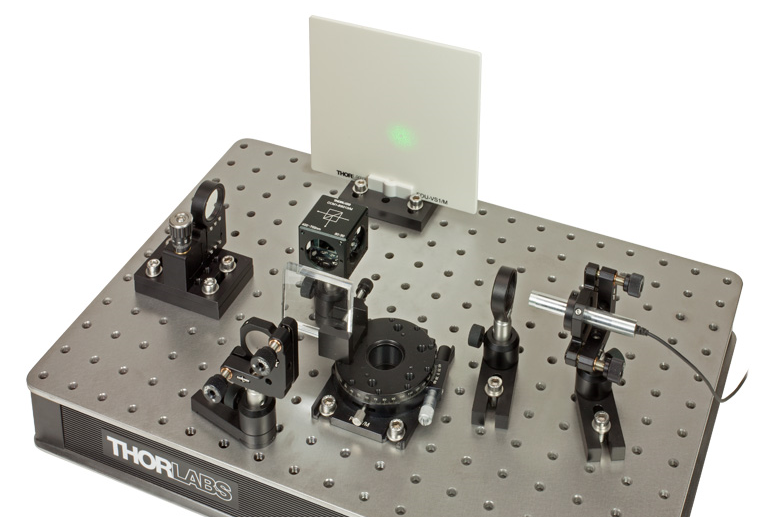
\includegraphics[width=0.5\textwidth]{./object/g11.png}};
					\node[] at (-3.25,1) {Miroir 1};
					\node[] at (-3,-1) {Miroir 2};
					\node at (0,3) {Écran};
					\node at (4.25,0.5) {Source Cohérente};
					\node at (-0.9,1.5) {Beam Splitter};
				\end{tikzpicture}
				\caption{Configuration de l'interféromètre de Michelson sur Kit ThorLabs}
			\end{figure}

		\section{Théorie et travail préparatoire}

			\subsection{Rappel théorique}

				\subsubsection{Figure d'interférence}

				Avant de commencer avec les manipulations on discutera brièvement la théorie de l'interféromètre de Michelson. On prendra comme référence le schema de la [Figure 2.1.], qui représente le chemin optique parcouru par les faisceaux dans l'interféromètre. Le faisceaux issu de la source laser est divisé spatialement en deux par le séparateur de faisceaux. Les deux faisceaux partiels se rencontrent à nouveau sur le séparateur après avoir été réfléchis par les deux miroirs perpendiculaires. La fonction principale du séparateur est la suivante: un faisceau lumineux est partiellement réfléchi et partiellement transmis à chaque fois. Ceci veut dire que sur l'écran, on aura globalement une fraction de l'énergie émise initialement par la source. On peut déduire mathématiquement comment l'intensité lumineuse qui arrive sur l'écran dépend de la différence $\Delta s$ entre les deux chemins optiques $s_1$ et $s_2$ parcouru par les deux faisceaux après le séparateur.

					\begin{figure}[!ht]
						\centering
						\begin{tikzpicture}
							\draw[black!70, thick] (0,-2) -- (0,2);
							\draw[black!40, thick] (-6,0) -- (6,0);

							\draw [-{Latex[length=3mm, width=2mm]}, black!40] (6,0) -- (3,0); 
							\draw [-{Latex[length=3mm, width=2mm]}, black!40] (0,0) -- (0,1.25);
							\draw [-{Latex[length=3mm, width=2mm]}, black!70] (0,0) -- (0,1);

							\draw[Latex-Latex] (0.5,-0.2) -- (0.5,-1.8);
							\draw[Latex-Latex] (-5.8,-0.75) -- (-0.2,-0.75);

							\filldraw[fill=gray!50] (-6.05,0.5) -- (-5.95,0.5) -- (-5.95,-0.5) -- (-6.05,-0.5) -- (-6.05,0.5);
							\filldraw[fill=gray!50] (-0.5,-1.95) -- (0.5,-1.95) -- (0.5,-2.05) -- (-0.5,-2.05) -- (-0.5,-1.95);
							\filldraw[fill=white] (6,0.25) -- (7.5,0.25) -- (7.5,-0.25) -- (6,-0.25) -- (6,0.25);
							\draw[very thick] (0.75,2) -- (-0.75,2);

							\filldraw[fill=black] (0.45,0.5) -- (0.5,0.5) -- (0.5,0.45) -- (-0.45,-0.5) -- (-0.5,-0.5) -- (-0.5,-0.45) -- (0.45,0.5);

							\node at (1.5,1.75) {Écran};
							\node at (-6,1) {Miroir 2};
							\node at (-1.25,-1.65) {Miroir 1};
							\node at (6.75,0.75) {Source cohérente};
							\node at (-1.5,0.5) {Beam Splitter};

							\node at (-3,-1) {$s_2$};
							\node at (0.75,-1) {$s_1$};

							

						\end{tikzpicture}
						\caption{Schéma qui montre le chemin optique parcouru par les deux faisceau sur les deux bras de l'interféromètre et qui ensuite vont interferer sur l'écran}
					\end{figure}

					On représente chaque faisceau lumineux incident sur l'écran comme une onde plane monochromatique:\\ $E_1=E_0\cos\left(\omega t-kx  \right) $ avec $i=1,2,\ldots$ où $\omega =\frac{2\pi c}{\lambda }$ et $k=\frac{2\pi}{\lambda }$ avec $\lambda $ étant la longueur d'onde de la source lumineuse. Les amplitudes des champs électriques des ondes $1$ et $2$ sur l'écran peuvent s'exprimer respectivement : 
					\begin{equation}
						\ds{E_1=\sqrt{RT} E_0\cos(\omega t + \varphi_1)}\quad\text{et}\quad E_2=\sqrt{RT} E_0\cos(\omega t+\varphi_2)
					\end{equation}	
					Où $R$ et $T$ sont respectivement les coefficients de réflexion et de transmission du séparateur de faisceaux, avec $\varphi_i = -ks_i = -\frac{2\pi s_i}{\lambda }$ la phase cumulée par l'onde sur le 'bras' $i$ de l'interféromètre, et $s_i$ étant la longueur du chemin parcouru par le faisceau $i$. Le produit $RT$ vient du fait que chaque faisceau qui arrive sur l'écran est une fois réfléchi, ou vice-versa. L'intensité totale sur l'écran sera donc donnée par : 
					\begin{equation}
						\ds{I(t)=\frac{1}{2}c\epsilon_0(E_1+E_2)^{2}=\frac{1}{2}c\epsilon_0RTE_{0}^{2}[\cos(\omega t +\varphi_1)+\cos(\omega t+\varphi_2)]^{2}}
					\end{equation}
					Naturellement nous pouvons détecter seulement la moyenne temporelle de l'intensité, on exprime donc celle-ci comme: 
					\begin{equation}
						\ds{\langle I\rangle} = \frac{1}{2}c\epsilon_0RTE_{0}^{2}\cdot \int\limits_{0}^{2\pi} [\cos(\omega t+\varphi_1)+\cos(\omega t+\varphi_2)]^{2} \  d (\omega t) = \frac{1}{2}c\epsilon_0RTE_{0}^{2}[1+\cos\left(\varphi_1-\varphi_2  \right) ]
					\end{equation}
					On assumera ici que $R=T=\frac{1}{2}$ par approximation du séparateur de faisceau, ainsi: 
					\begin{equation}
						\ds{\left<I \right> \frac{1}{4}}c\epsilon_0E_{0}^{2} \left[ 1+\cos\left(\Delta\varphi  \right)  \right]  		
					\end{equation}
										Avec: \\\vspace{2mm}
					\centerline{$\ds{\Delta\varphi=\frac{2\pi}{\lambda}\Delta s}$}
					Où $\ds{\Delta s = s_1-s_2}$ est la différence de marche entre les deux faisceaux qui interfèrent. L'intensité sur l'écran au centre de la figure d'interférence est donc une fonction sinusoïdale de la différence de phase ou de chemin optique entre les ondes parcourant les deux bras de l'interféromètre. Cela est montré dans la [Figure 2.2.]. 

					\begin{figure}[ht!]
						\centering
						\begin{tikzpicture}
							\begin{axis}[grid=none, axis lines=middle,
								width=10cm, height=4cm,
								xmin=0,xmax=10,
								ymin=0,ymax=1.25,
								xtick={1.57,3.14,4.71,6.28,7.85,9.42},
								xticklabels={$\frac{\pi}{2}$,$\pi$,$\frac{3\pi}{2}$,$2\pi$,$\frac{5\pi}{2}$,$3\pi$}]
								
								\draw[color=blue, domain=0:10, samples=100]   plot (\x,{0.5*cos(\x r)+0.5});
										
							\end{axis}
						\end{tikzpicture}
						\caption{Variation de l'intensité lumineuse au centre de la figure d'interférence en fonction de la différence de phase entre les deux faisceaux qui arrivent sur l'écran}

					\end{figure}

					Il est important de comprendre que la formule (2.4) et le graphique de la [Figure 2.2.] donnent la variation de l'intensité sur l'écran au centre de la figure d'interférence lorsque on change la longueur relative entre les deux bras de l'interféromètre. Toutefois la distribution spatiale d'intensité observé sur l'écran pour une valeur donné de $\ds{\Delta s}$ est une figure étendue transversalement à cause de la divergence des faisceaux lumineux, et elle est formé par des anneaux concentriques.

					Dans ce cas la position des franges brillantes sur l'écran sera donné par la relation : \\\vspace{2mm}
					\centerline{$\ds{X_m=D\sqrt{2-m\frac{\lambda}{AB}}\quad \text{avec}\quad m=0,\pm 1,\pm 2}$}

					Où $D$ est la distance des sources de l'écran, $AB\ll D$ de façon à ce que les deux sources puissent être confondues.

					Lorsque l'un des deux miroirs est tourné légèrement, le front d'onde qui provient de ce miroir change et donc la figure d'interférence résulte altérée. Dans la [Figure 2.3.] on montre comme la figure d'interférence change lorsqu'un miroir est tourné par rapport à sa position perpendiculaire initiale.

					\begin{figure}[ht!]
						\centering
						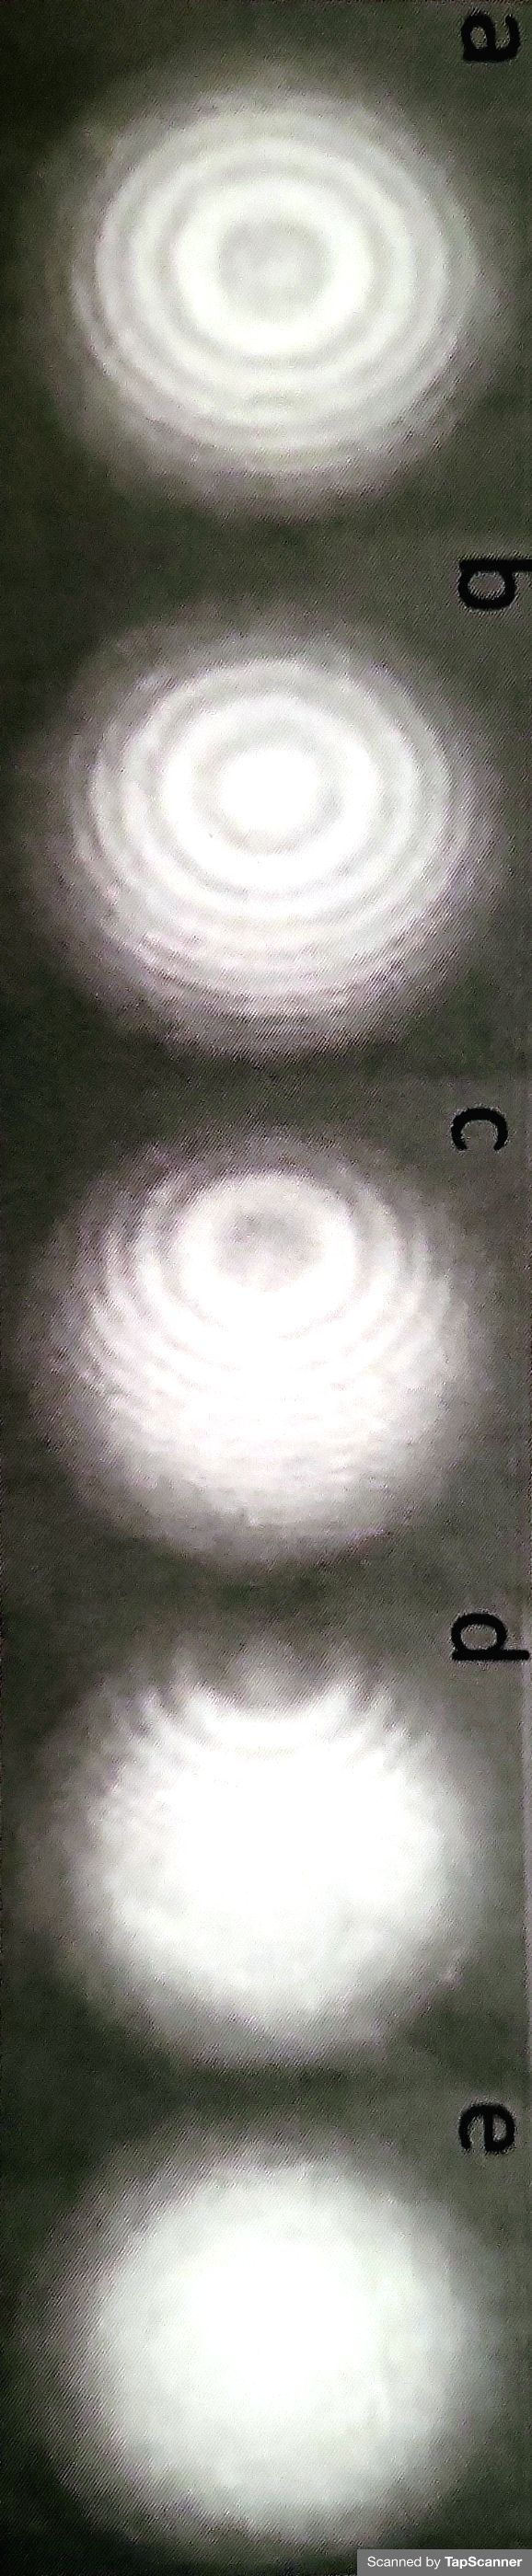
\includegraphics[width=0.15\textwidth,angle=90, origin=c]{./object/g3.jpg}	
					\end{figure}
					\vspace{-5.2cm}
					Figure 2.3. Variation de la figure d'interférence lorsqu'un des miroirs est tourné par rapport à sa position perpendiculaire initiale	
					
					A un premier regard on pourrait penser que la figure d'interférence translate tout simplement sur l'écran. En réalité ce n'est pas le cas, et pour voir il suffit de comparer les [Figures 2.3.a et 2.3.b]. Ce qu'il se passe en réalité est que lorsque on tourne le miroir la frange centrale passe par des maxima et des minima d'intensité et la distance entre deux franges brillantes successives, c'est de cette façon qu'il faut voir les choses.

					\subsubsection{Cohérence}

					La cohérence dans le sens le plus large, décrit la capacité de la lumière de créer de l'interférence. L'intervalle temporel maximum $\Delta t_c$ pendant lequel la différence de phase entre ondes partielles aléatoires, à un point donné, varie de moins de $2\pi$ est appelé 'temps de cohérence'. Dans ce cas, si la différence est inférieure à $2\pi$ on dira que les ondes partielles sont temporellement cohérentes.

					On peut imaginer par exemple que ces ondes partielles soient les harmoniques qui composent la lumière provenant d'une source spectralement large, comme montré dans la figure 6a. Dénotons sa largeur spectrale avec $\Delta \nu$. Si $\nu_0$ indique la fréquence centrale, alors la lumière émise par la source peut être vue comme la superposition d'ondes partielles avec des fréquences comprises dans l'intervalle $\ds{\left[ \nu_1=\nu_0-\frac{\Delta\nu}{2}, \nu_2=\nu_0+\frac{\Delta\nu_0}{2} \right] }$ 

					Si la différence de phase entre les ondes de fréquence $\nu_1$ et $\nu_2$ à l'instant $t=0$ est égale à zéro, alors à un instant $t>0$ quelconque elle sera donnée par: 
					\begin{equation*}
						\ds{\Delta\varphi(t)=2\pi(\nu_2-\nu_1)t}
					\end{equation*}
					Le temps de cohérence peut être alors calculé en imposant que $\ds{\Delta\varphi(\Delta t_c)=2\pi(\nu_2-\nu_1)\Delta t_c=2\pi}$, ce qui donne: 
					\begin{equation*}
						\ds{\Delta t_c=\frac{1}{\Delta\nu}}
					\end{equation*}
					Où $\ds{\Delta\nu=\nu_2-\nu_1}$ est la largeur spectrale de la source. Lié au concept de temps de cohérence il y a le concept de 'longueur de cohérence', c'est à dire le chemin $\Delta l_c$ que la lumière peut parcourir pendant l'intervalle temporel de cohérence: 
					\begin{equation*}
						\ds{\Delta l_c=c\Delta t_c}
					\end{equation*}
					Où $c$ dénote la vitesse de la lumière. Dans le cadre d'interférence produites avec un interféromètre, le concept de longueur de cohérence est facilement compréhensible: si la différence entre les bras de l'interféromètre dépasse la demi - longueur de cohérence aucune interférence ne sera observée. Pour une utilisation plus pratique des concepts de temps et de longueur de cohérence, il est plus simple de les exprimer en fonctions des longueurs d'ondes: 
					\begin{equation*}
						\ds{\Delta \nu=\nu_2-\nu_1=\frac{c}{\lambda_2}-\frac{c}{\lambda_1}=\frac{c(\lambda_1-\lambda_2)}{\lambda_1\lambda_2}=\frac{c\Delta\lambda}{\lambda1\lambda_2}\approx \frac{c\Delta\lambda}{\lambda_{0}^2}}
					\end{equation*}
					Avec: 
					\begin{equation*}
						\begin{aligned}
							\begin{cases}
								\Delta t_c \approx \frac{\lambda_{0}^2}{c\Delta\lambda}\\
								\noalign{\vskip9pt}
								\Delta l_c \approx \frac{\lambda_{0}^2}{\Delta\lambda}
							\end{cases}							
						\end{aligned}
					\end{equation*}

			\section{Test et mesures}
			
				\subsection{Tests préliminaires}

					En prenant la configuration de l'interféromètre de Michelson on allume la source de laser et on s'assure qu'une figure d'interférence apparaisse sur l'écran en manipulant légèrement les visses de réglage des miroirs pour la centrer.

					Pendant ces manipulation préliminaires on remarque qu'en faisant varier la distance antre le miroir 1 et le séparateur que la figure d'interférence semble agrandir ou diminuer le nombre de franges circulaire concentriques. Ceci est logique car on fait donc varier la distance de marche $\Delta s$ induisant un décalage de phase $\Delta\varphi$ dans la figure de répartition d'intensité (Eq 2.4).

					On remarque de plus qu'il y a une deuxième figure d'interférence qui ce situe au niveau du laser et en regardant scrupuleusement on s'aperçoit que l'interférence n'est pas exactement la même. Ceci vient du fait que le séparateur laisse un partie de la lumière à âtre redirigé vers l'écran mais aussi une autre partie vers le laser en raison des miroirs. Le soucis c'est que le laser n'emprunte pas le même chemin pour ces deux figures d'interférence, c'est pour ça que l'on voit qu'elle n'ont pas la même interférence. On peut voir ceci sur la [Figure 3.1] 

					\begin{figure}[ht!]
						\centering
						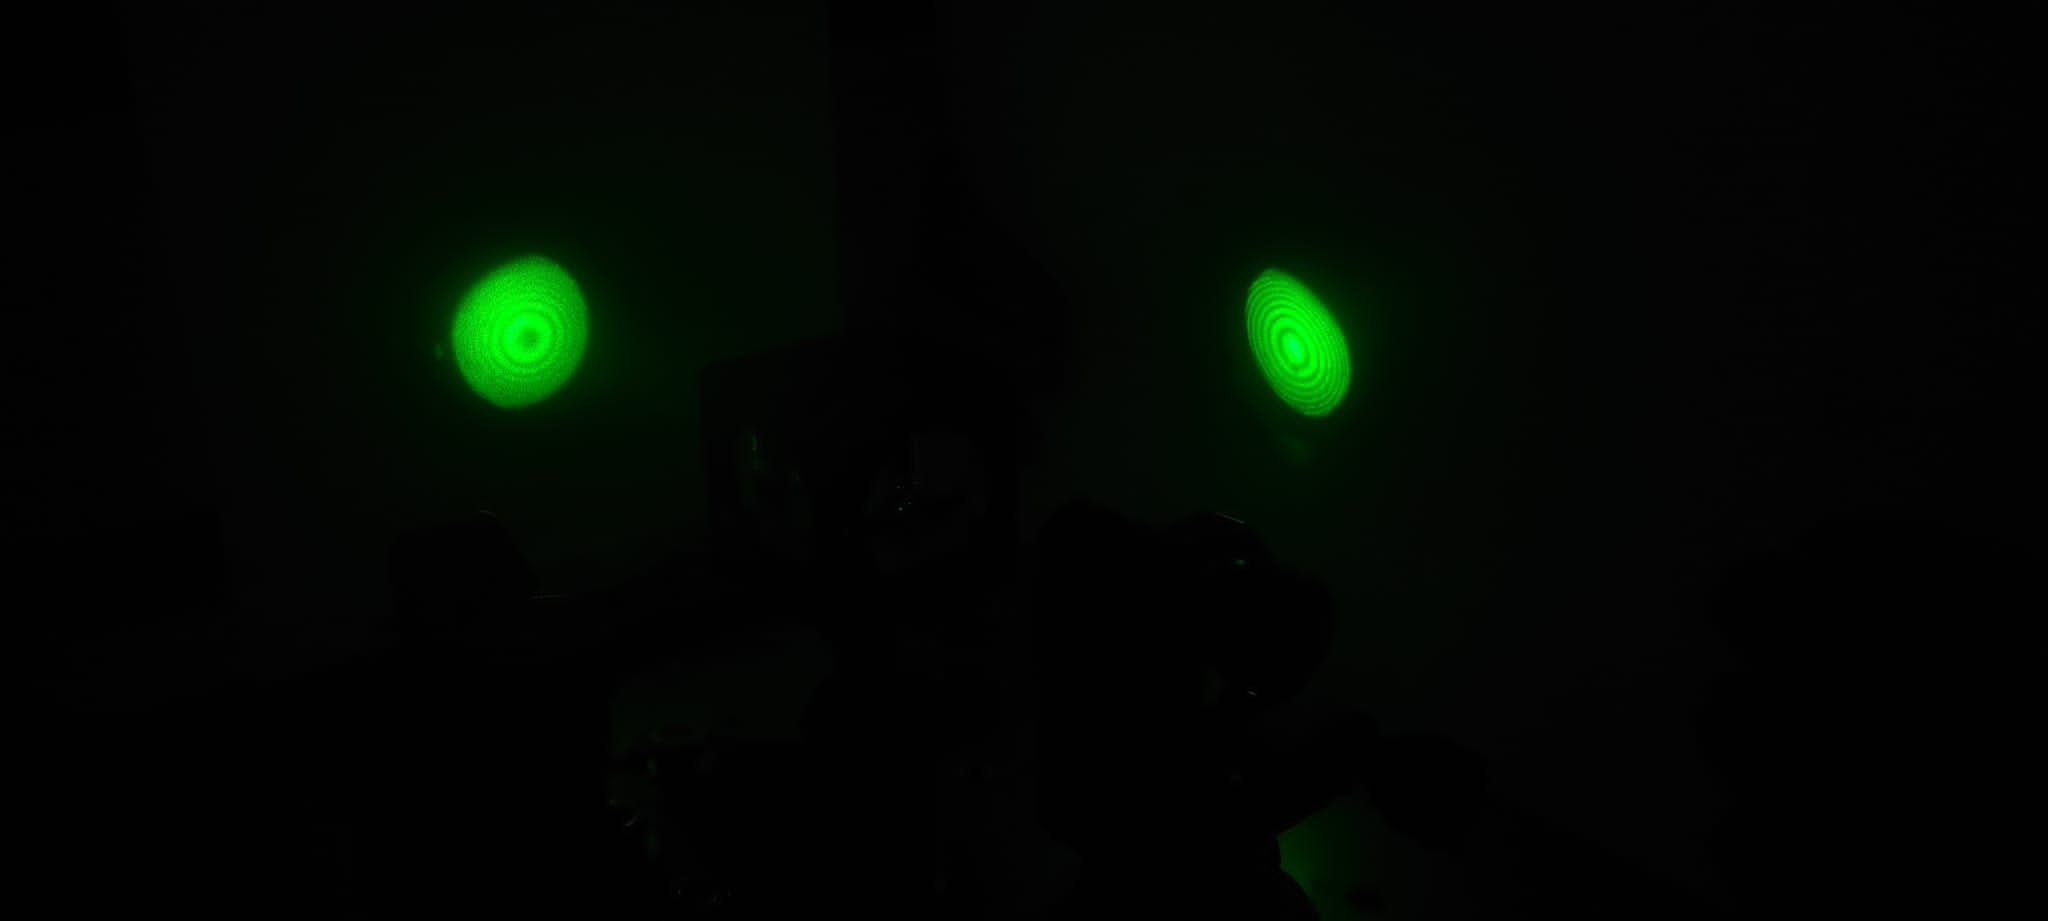
\includegraphics[width=0.6\textwidth]{./object/g4.jpg}
						\caption{Figure d'interférence observé au niveau de l'écran et au niveau du laser}
					\end{figure}

				\subsection{Détermination de la longueur d'onde de la source laser}

					L'équation (2.4)  et la [Figure 2.2.] offrent une façon élégante pour mesurer la longueur d'onde d'une source lumineuse monochromatique, comme le laser. Lorsque l'un des miroirs est translaté la différence de longueur entre les bras de l'interféromètre change; en conséquence la différence de marche entre les faisceaux change ce qui fait varier la figure d'interférence. Comme on peut remarquer dans le graphique de la [Figure 2.2] une transition d'un maximum au successif correspond à un changement de différence de marche de $\lambda$. Si en translatant le miroir d'une quantité $\Delta x$ on observe $N$ transitions alors on peut écrire : 
					\begin{equation}
						\ds{\Delta s = 2\Delta x = N\lambda \implies \lambda=\frac{2\Delta x}{N}}
					\end{equation}
					En utilisant ce concept on peut alors mesurer la longueur d'onde de la source laser utilisé. On réalise ainsi une mesure pour un déplacement $\Delta x = 25\pm 0.1\ \mu m$, dans lequel on compte 97 transitions successives, ainsi en se reposant sur l'équation (2.5) on retrouve $\lambda=515\pm 20\ nm$ ce qui équivaut à un erreur de 3.8\%.

				\subsection{Détermination du coefficient  de dilatation thermique de l'aluminium}

					Dans cette experience on utilise l'interféromètre pour mesurer le coefficient de dilatation thermique de l'aluminium.

					On commence par remplacer le miroir 1 par un dispositif de mesure de dilatation thermique en veillant à ce que le miroir soit bien perpendiculaire au faisceau laser. On ajuste ensuite en utilisant les visses sur le miroir 2 la position de la figure d'interférence sur l'écran. Ensuite un insère une tige d'un thermomètre à l'intérieur du barreau d'aluminium afin de relever sa température. On branche ensuite les contactes de la barre d'aluminium sur un générateur de tension de façon à pour chauffer la barre en utilisant la resistance propre au barreau.

					En applicant cette tension la température du barreau augmente ce qui entraine alors sa dilatation et le déplacement du miroir. Cela provoque un certain nombre de transition de franges qui peuvent être observées sur l'écran. On compte alors le nombre de transitions à partir du moment où l'on applique de la tension jusqu'au moment où la température se stabilise. On procède ainsi pour des valeurs de $5V$, $7V$ et $9V$.

					\begin{figure}[ht!]
						\centering
						\begin{tabular}{|c|c|c|c|c|c|}
							\hline
							Tension & $T_i$ & $T_f$ & $\Delta T$ & $\Delta x$ & Longueur\\
							\hline
							$4.4V$ & $21\pm 0.5^{\circ}$ & $27 \pm 0.5^{\circ}$ & $6\pm 1^{\circ}$ & $13.1\pm 0.5\ \mu m$ & $90013.1\pm 0.5\ \mu m$\\
							\hline
							$7V$ & $27\pm 0.5^{\circ}$ & $38\pm 0.5^{\circ}$ & $11\pm 1^{\circ}$ & $18.8\pm 0.75\ \mu m$ & $90018.8\pm 0.75\ \mu m$\\
							\hline
							$8.8V$ & $38\pm 0.5^{\circ}$ & $49\pm 0.5^{\circ}$ & $11\pm 1^{\circ}$ & $21.1\pm 0.82\ \mu m$ & $90021.1\pm 0.82\ \mu m$\\
							\hline
						\end{tabular}
						\caption{Tableau de mesure obtenu lors de la réalisation de l'expérience}
					\end{figure}

					\begin{figure}[ht!]
						\centering
						\begin{tikzpicture}[]
							\begin{axis}[
								xmin= 0, xmax= 30,
								ymin= 90000, ymax = 90025,
								ytick={90005,90010,90015,90020},
								yticklabels={9.0005,9.0010,9.0015,9.0020},
								xlabel={Variation de température $\Delta T$ $[^{\circ}C]$},
								ylabel={Longueur du barreau $L$ $[\mu m]$},
								width = 0.5\textwidth,
								height = 0.3\textwidth,
								grid= both,
								legend pos=south east,
								legend cell align = left,
								error bars/x dir=both,
								error bars/y dir=both,
								error bars/x explicit,
								error bars/y explicit,
							]
							\addplot[blue, only marks, mark=x, mark size=3pt] table[x={x}, y={y}, column sep = space, y error=yer, x error=xer] {./object/d3.txt};
							\addplot[blue,smooth,domain=0:30,samples=100] {0.363636*x+90011.48};
							\addplot[blue,dashed,smooth,domain=0:30,samples=100] {0.274409*x+90009.76};
							\addplot[blue,dashed,smooth,domain=0:30,samples=100] {0.452863*x+90013.19};


							\node at (20,90010) {\blu$y=0.363636x+90011.5$};
							\legend{\small Mesures, \small Courbe de tendance};

							\end{axis}

						\end{tikzpicture}
						\caption{Relation illustrant la dilatation thermique de l'aluminium}
					\end{figure}
					\newpage
					On retrouve ainsi un coefficient de dilatation thermique de $4.0404\pm 0.99141\ [10^{-6}] ^{\circ}\ C^{-1}$ ce qui est relativement proche de la valeur attendue à $26\ \cdot 10^{-6} ^{\circ}\ C^{-1}$ mais $6.5$ fois plus petite. 

					On ne néglige pas la possibilité d'erreur de mesure cependant les valeurs obtenues sont conformes au coefficient de dilatation trouvé. On conclut donc que cet écart doit provenir d'un défaut materiel où d'une erreur d'interprétation.

				\subsection{Interférences avec une source LED cohérente}

					Puisque la LED est une source spectralement large, pour produire une figure d'interférence sur l'écran avec une LED, les bras de l'interféromètre doivent avoir a peu près la même longueur. Si la différence de longueur est telle que la longueur de cohérence est dépassé, aucune figure d'interférence ne sera observée comme nous pouvons le constater ci-dessous.

					\begin{figure}[ht!]
						\centering
						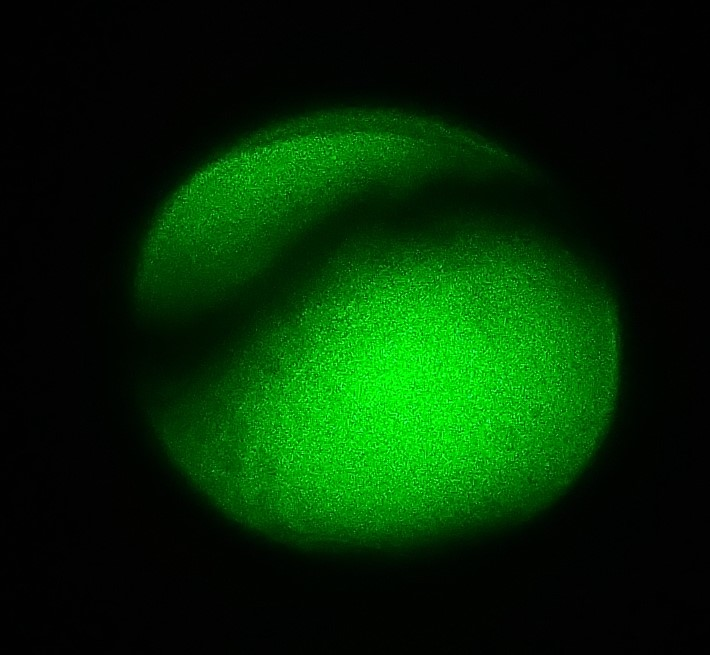
\includegraphics[width=0.2\textwidth]{./object/g5.jpg}
						\caption{Perte de la figure d'interférence caractéristique de la configuration de Michelson}
					\end{figure}

					Cependant puisqu'il existe toujours une différence de positionnement transversale on se situe donc dans une configuration similaire au fentes de Young, c'est à dire qu'il est possible d'observer des franges rectilignes uniformes. 

					\begin{figure}[ht!]
						\centering
						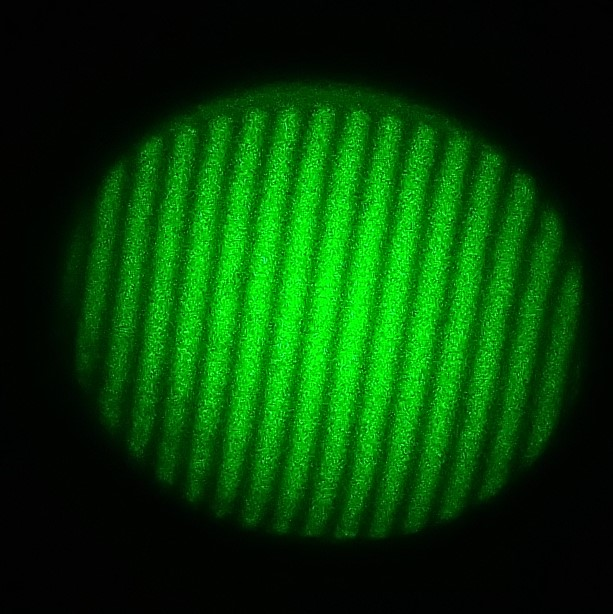
\includegraphics[width=0.2\textwidth]{./object/g6.jpg}
						\caption{Figure d'interférence similaire au fentes de Young}
					\end{figure}

					Une fois que l'on a retrouvé cette figure d'interférence on se propose alors de trouver la longueur de cohérence associé à la LED rouge.

					Pour ceci on mesure il faut determiner la largeur de l'interfrange et la multiplier par la distance de marche.

					Cependant il reste encore possible de comparer la longueur de cohérence en analysant la figure d'interférence des deux sources:

					\begin{figure}
						\centering
						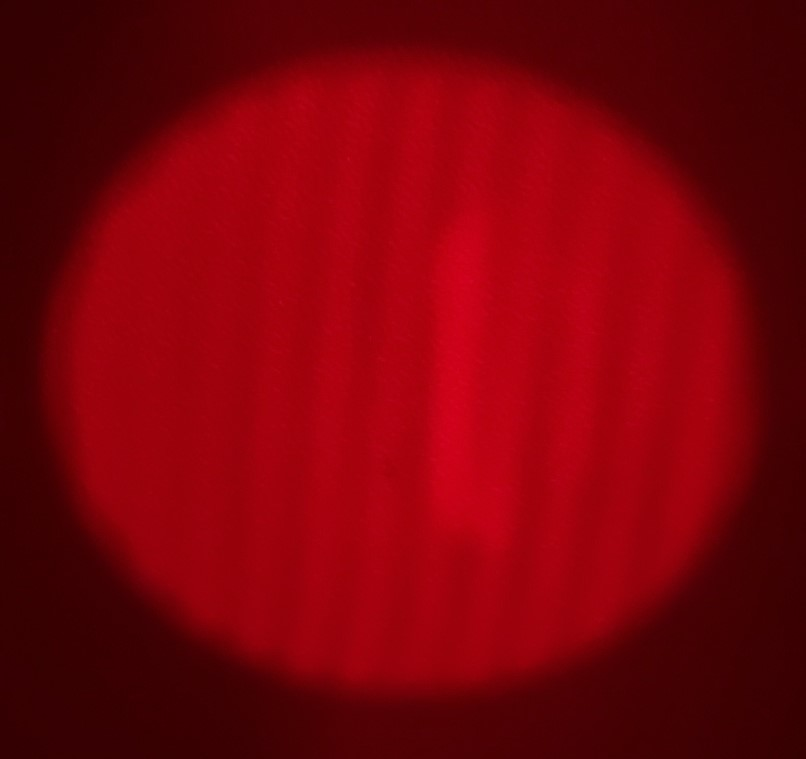
\includegraphics[width=0.2\textwidth]{./object/g7.jpg}
						\hspace{2cm}
						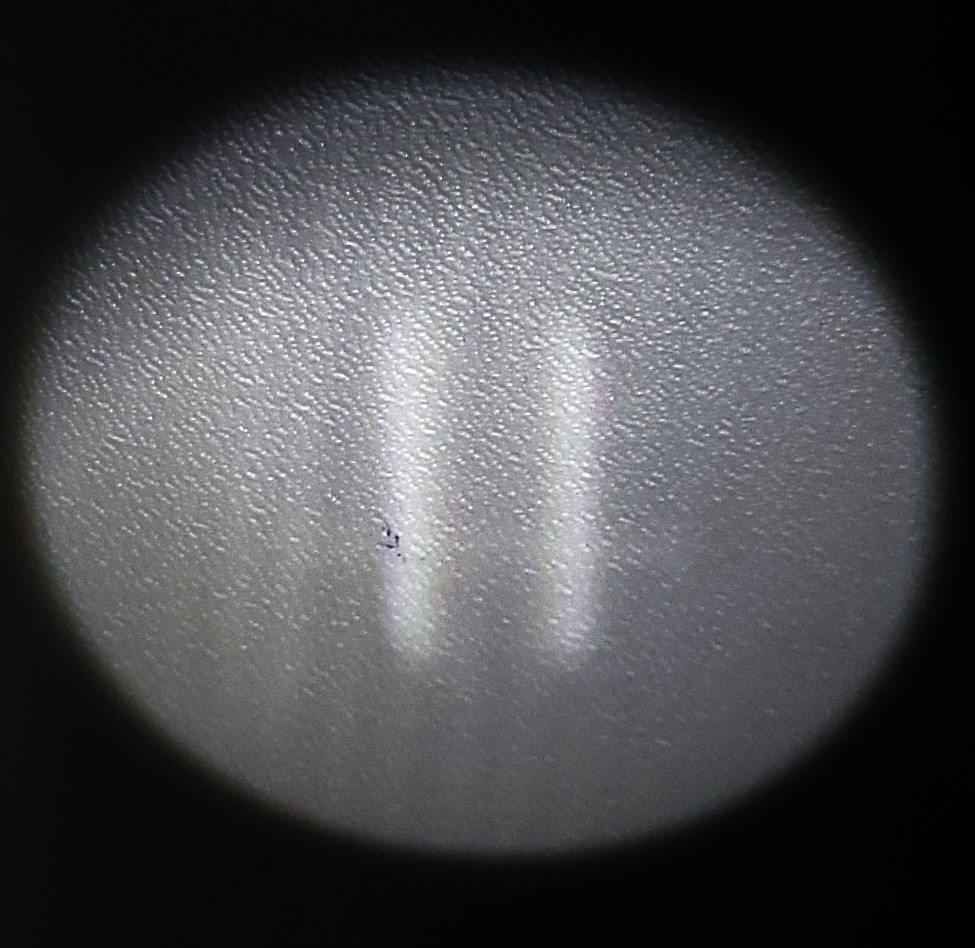
\includegraphics[width=0.2\textwidth]{./object/g8.jpg}
						\caption{Interférence des deux LEDs}
					\end{figure}

					On constate que la largeur de la plage d'interférence est nettement plus grande pour la LED rouge mesuré à $\left[ 5\ \mu m;32\ \mu m \right] $, tandis que la plage d'interférence pour la LED blanche n'est qu'à $\left[ 14\ \mu m;23\ \mu m \right] $. On observe donc que la lumière blanche a donc une largeur spectrale plus grosse ce qui affecte directement la plage d'interférence, ainsi on peut donc conclure que la LED rouge a une longueur de cohérence plus grande que la LED blanche.






















				
				




    

\end{document}
